\chapter{Introduction} % senza numerazione
\label{cha:intro}

\section{Summary}

The goal of this project, as described in abstract, aims to develop a complete system for \textbf{surveillance purposes} using ground robots, but also flying ones. Since the project is quite complex, it is \textbf{shared} between other two students, with each one of us focusing on his subproject.

\bigskip

\begin{figure}[h]
  \centering
  \begin{tikzpicture}
    \node[title] (webinterface-inner) {Web interface};
    \node[rectangle, draw, rounded corners, fit=(webinterface-inner)] (webinterface) {};
    \node[intro, left=of webinterface] (hidden-task-1) {};
    \node[intro, right=of webinterface] (hidden-task-2) {};
    \node[cloud, below=4em of webinterface, draw, aspect=2] (planning) {Planning};

    \node[mine, left=of planning] (ugv) {UGVs controller};
    \node[info, above=3em of ugv] (ugv-data) {\textbf{Initial pose \& Lidar data}};
    \node[intro, below=3em of ugv] (ugv-image) {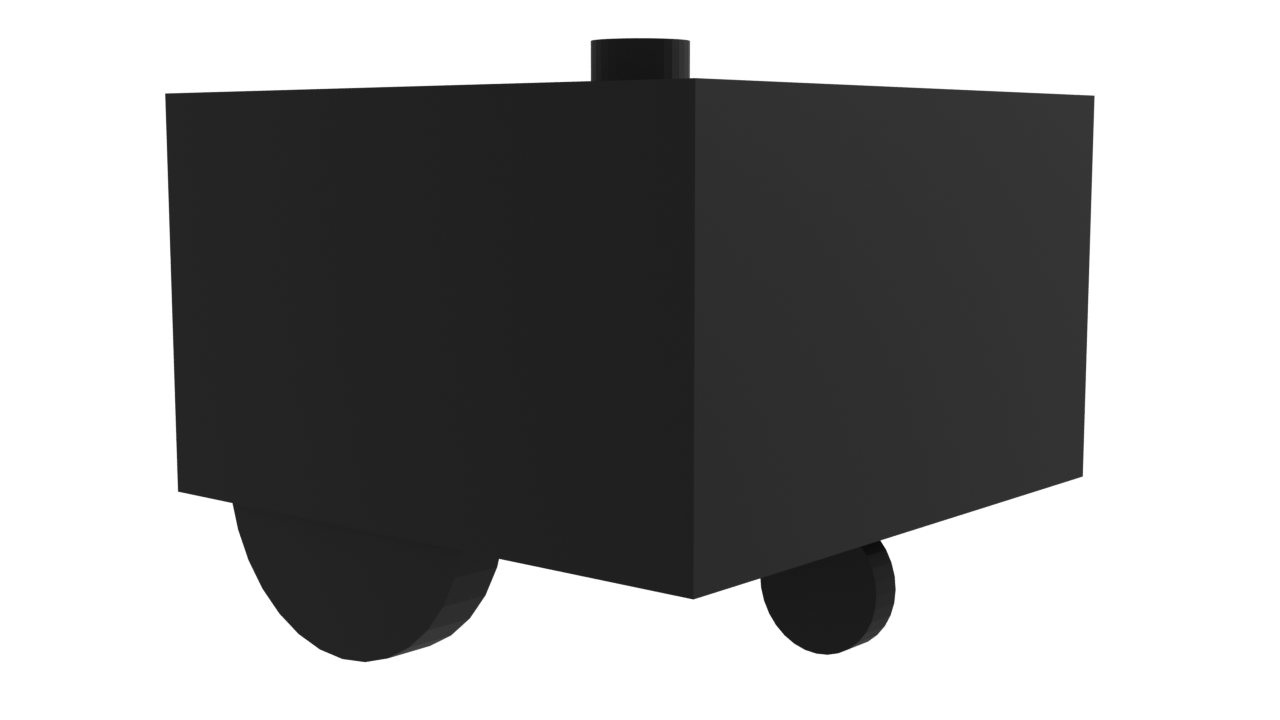
\includegraphics[width=0.2\textwidth]{images/ugv}};

    \node[title, right=of planning] (uav) {UAVs controller};
    \node[info, above=3em of uav] (uav-data) {\textbf{Motion-capture \& GPS data}};
    \node[intro, below=3em of uav] (uav-image) {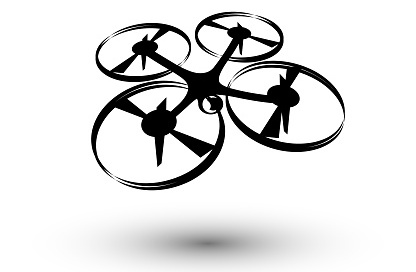
\includegraphics[width=0.2\textwidth]{images/uav}};

    \draw[arrow] (webinterface) -- node [right] {\textit{interacts with}} (planning);
    \draw[arrow] (hidden-task-1) -- node [above] {tasks} (webinterface);
    \draw[arrow] (hidden-task-2) -- node [above] {tasks} (webinterface);

    \draw[arrow] (planning) -- node [above] {\textit{dispatches to}} (ugv);

    \draw[arrow] (ugv-data) -- node [left] {\textit{is passed to}} (ugv);
    \draw[arrow] (ugv) -- node [right] {\textit{commands}} (ugv-image);

    \draw[arrow] (planning) -- node [above] {\textit{dispatches to}} (uav);

    \draw[arrow] (uav-data) -- node [right] {\textit{is passed to}} (uav);
    \draw[arrow] (uav) -- node [left] {\textit{commands}} (uav-image);

  \end{tikzpicture}
  \caption{Project architecture. The node with the thick border is the one discussed in this thesis}
  \label{fig:project}
\end{figure}

\bigskip

As shown in \autoref{fig:project}, it is subdivided as follows: 

\begin{itemize}
  \item a \textbf{planning system} with a \textbf{web interface}, responsible for dispatching surveillance tasks to \acrfull{ugvs} and/or \acrfull{uavs} the best possible way, according to their battery charge, providing them with some waypoints to reach; 
  \item a solution to independently control drones (\textbf{\acrshort{uavs} controller});
  \item a solution to independently control ground robots, avoiding obstacles (\textbf{\acrshort{ugvs} controller});
\end{itemize}

Everything is developed using \acrfull{ros}2, that gives us the opportunity to work \textbf{separately} on our subproject, and thanks to its \textbf{modularity}, in the end we will just have to put them all together.

The reason why I chose the internship and this resulting thesis, is driven by my \textbf{growing interest} in this topic: just a few months before taking part in this work, I attended a course on \textit{robotic fundamentals}\cite{intro2robotics} where we also developed a project quite similar to this, but with a robotic manipulator.

For me, the intriguing part is the possibility of giving some inanimate object, like a wheeled robot or a manipulator, something that could be described as \textbf{intelligence}, the ability to perform certain tasks in response to others, and figure out which ones are the \textbf{best suited} for each particular situation. The challenges I decided to face are: working for the first time on a \textbf{mobile robot} and choosing the \textbf{new version} of \acrshort{ros}, with some improvements compared to the previous one, but with less support from the community.

\section{Other projects involved}

What follows is a brief description of the work done by the other two students to get a better and clear idea of the workflow of the whole system.

\subsection{Planning system, fleet management and web interface}
\label{sub:planning}

It is brain of the system and it allows the user to choose which type of robot he wants to use (only ground robots or drones with ground robots as auxiliaries), and then it dispatches the tasks to the right robots. You can define multiple goal for each robot, and once done, the planning system will begin to figure out the best way to organize the fleet.

In order to resolve a problem you must have defined a \textbf{domain}: this contains a description of action space you are interested in, in which you could specify \textbf{reachable targets}, making use of a set of \textbf{predefined actions}, that require certain \textbf{preconditions} to be fulfilled before they are executed and that cause \textbf{changes} to the environment. In order to solve a problem, it is necessary to verify if its domain is \textbf{compatible} with the planning one, or in other words, if the goal is achievable, and in this case you can look for a \textbf{solution} (i.e., a sequence of actions to be performed).

Each robot waits for new commands to be received and performs a specific action based on task required. Here follows a list of tasks:

\bigskip

\begin{minipage}[h]{0.45\textwidth}
  \centering
  \textbf{\acrshort{uavs} actions}
  \begin{itemize}
    \centering
    \item \code{uav\_move}
    \item \code{uav\_take\_photo}    
    \item \code{uav\_land\_on\_ugv}
    \item \code{uav\_take\_off\_ugv}
  \end{itemize}
\end{minipage}
\begin{minipage}[h]{0.45\textwidth}
  \centering
  \textbf{\acrshort{ugvs} actions}
    \begin{itemize}
      \centering
      \item \code{ugv\_move}
      \item \code{ugv\_charge}
      \item \code{try\_ugv\_charge}
      \item \code{ugv\_transporting\_uav\_move}
    \end{itemize}
\end{minipage}

\bigskip

These actions are the only actions that the planning system uses when a problem is specified, to find a possible result: the output are \textbf{cascading actions} that will have to be performed, and when one is completed you can move on to the next. The implementation is left to those who work on that robot, because of their \textbf{better understanding} of its architecture.

But, speaking of movement, we need \textbf{coordinates}. These are extracted from the 3D mesh and thanks to an \textbf{annotation program} you can give them a name: in this way, instead of using a bunch of numbers, you use the name of the room, and their relationship is defined in a file. Each room is then \textbf{connected} to the others by default.

Thanks to a web interface, communicating with \acrshort{ros}2 via \textbf{rosbridge} (using \textbf{websockets}), the user can define where the robots are initially are and where they should go, and by pressing just one button they will start moving.   

\subsection{Drones control}

This project aims to control the drones \textbf{autonomously}: in order to do this, the drones are equipped with an \textbf{autopilot module} called \textit{Pixhawk 4}. In such a manner you do not have to control the drones \textbf{manually} (i.e. setting the motors speed), but you can simply send commands (e.g. move forward or backward, turn left or right) and the autopilot will do the rest. Fortunately, there is a \textbf{bridge} that allows communication between this module and \acrshort{ros}2, so you will be able to create subscribers and publishers that interface \textbf{directly} with \textbf{PX4 UORB topics}\cite{px4}.

The main command that is continuously sent is called \textbf{offboard}: it let the drone know there is still someone who wants to control it, otherwise it will land, for security reasons. The other command is \textbf{TrajectorySetPoint} which allows you to set the target position and orientation of the drone; then, the initial and final positions are \textbf{interpolated} with a \textbf{Catmull-Rom spline}, in order to have a smoother trajectory.

The drone uses \textbf{GPS} to know where it is, but for real-world testing purposes, the chosen room could not provide the necessary signal, so \textbf{OptiTrack cameras} were used to simulate it. Thanks to some \textbf{reflective surfaces}, the eight cameras can \textbf{estimate} the drone position and orientation, providing a \textbf{temporary alternative} to GPS data, which only works within a limited space.

But, before testing the drone in the real world, with possible catastrophic consequences, it is important to be sure that it works at least in a \textbf{simulation}; here Gazebo\footnote{A simulation suite, will be well described in \autoref{sec:gazebo}} comes to the rescue. When testing with Gazebo, only position information can be read without problems from the interface provided by the program itself, while the orientation one comes from the controller bridge: these data are then fused together inside a node and sent to the drone to give it feedback of its actions\footnote{This is called \textbf{odometry}}. Speaking of the real environment, if the GPS is available, it will be possible to get information about the position and orientation directly from the drone, so the setup is almost the same. 

With everything put together, the drone can be controlled autonomously.

\subsection{Thesis outline}

This thesis is structured as follows:
\begin{itemize}
  \item \textbf{\autoref{cha:techstack}} describes software and libraries employed in the system development, for a better understanding;
  \item \textbf{\autoref{cha:realworld}} shows the necessary steps to implement the system with real robots;
  \item \textbf{\autoref{cha:simworld}} covers the simulation part, developing both a simulated environment and a robot;
  \item \textbf{\autoref{cha:navigation}} introduces the navigation system and shows how it is applied to this project;
  \item \textbf{\autoref{cha:planningbridge}} describes how the planning part has been integrated with everything else, with the help of custom bridge nodes;
  \item \textbf{\autoref{cha:futureworks}} discusses possible developments and improvements.
\end{itemize}